\documentclass[11pt,letterpaper]{article}
\usepackage[utf8]{inputenc}
\usepackage[left=1in,right=1in,top=1in,bottom=1in]{geometry}
\usepackage{amsfonts,amsmath}
\usepackage{graphicx,float}
\usepackage{csquotes}
% -----------------------------------
\usepackage{hyperref}
\hypersetup{%
  colorlinks=true,
  linkcolor=blue,
  citecolor=blue,
  urlcolor=blue,
  linkbordercolor={0 0 1}
}
% -----------------------------------
\usepackage[style=authoryear-icomp,backend=biber]{biblatex}
\addbibresource{citation.bib}
% -----------------------------------
\usepackage{fancyhdr}
\newcommand\course{MATH-UA.0263\\Partial Differential Equations}
\newcommand\hwnumber{8}                  % <-- homework number
\newcommand\NetIDa{Ryan Sh\`iji\'e D\`u} 
\newcommand\NetIDb{March 31st, 2023}
\pagestyle{fancyplain}
\headheight 35pt
\lhead{\NetIDa\\\NetIDb}
\chead{\textbf{\Large Worksheet \hwnumber}}
\rhead{\course}
\lfoot{}
\cfoot{}
\rfoot{\small\thepage}
\headsep 1.5em
% -----------------------------------
\usepackage{titlesec}
\renewcommand\thesubsection{(\arabic{section}.\alph{subsection})}
\titleformat{\subsection}[runin]
        {\normalfont\bfseries}
        {\thesubsection}% the label and number
        {0.5em}% space between label/number and subsection title
        {}% formatting commands applied just to subsection title
        []% punctuation or other commands following subsection title
% -----------------------------------
\setlength{\parindent}{0.0in}
\setlength{\parskip}{0.1in}
% -----------------------------------
\input{../command.tex}
\begin{document}

\section{Alternative formula for Fourier transform}
In the HW you have one definition of the Fourier transform and its associated inversion formula:
\begin{align}
    &\hat f(\xi) = \int f(x)e^{-i\xi x} \;\de x,\\
    &f(x) = \int \hat f(\xi)e^{+i\xi x} \;\de \xi \cdot\frac{1}{2\pi}.
\end{align}
An alternative formula that absorbs the $2\pi$ factor into the Fourier kernal is:
\begin{align}
    &\hat f(\xi ) = \int f(x)e^{-2\pi i\xi x} \;\de x,\\
    &f(x) = \int \hat f(\xi)e^{+2\pi i \xi x} \;\de \xi \label{eq:Four_inv}.
\end{align}
Show that they are equivalent. I would use the second version in this note.

\section{Poisson summation formula}
[From \S5.3 of \cite{SteinShakarchi_03}] Given a Schwartz function $f$ on the real line, we can construct a new periodic (with period 1) function on the circle by the recipe
\begin{align}
    F_1(x) = \sum_{n=-\infty}^\infty f(x+n).
\end{align}
Another way is by Fourier analysis. Start with \eqref{eq:Four_inv} and consider its discrete analogue, where the integral is replaced by a sum:
\begin{align}
    F_2(x) = \sum_{n=-\infty}^\infty \hat f(n)e^{2\pi inx}.
\end{align}
A technical note, both of these sum are convergent absolutely and uniformly (for any compact interval) because of the assumption that $f$ is in the Schwartz space. Therefore, they are continuous. 

\subsection{}
Show that the two approaches are the same. That is, show the Poisson summation formula
\begin{align}
    \sum_{n=-\infty}^\infty f(x+n) = \sum_{n=-\infty}^\infty \hat f(n)e^{2\pi inx}.
\end{align}
In particular we have the corollary
\begin{align}
    \sum_{n=-\infty}^\infty f(n) = \sum_{n=-\infty}^\infty \hat f(n).
\end{align}

Hint: Show both sides (which are periodic) have the same Fourier series. Then the function is the same because Fourier series are unique for continuous function.

\subsection{Heat kernels} We have the heat kernel for the heat equation (with coefficient 1) on $\mathbb{R}$:
\begin{align}
    \mcal{H}_t(x) = \frac{1}{(4\pi t)^{1/2}}e^{-x^2/4t}
\end{align}
which has the Fourier transform
\begin{align}
    \hat{\mcal{H}}_t(\xi) = e^{-4\pi^2 \xi^2 t}.
\end{align}
You also derived the heat kernel on a periodic interval of length 1:
\begin{align}
    H_t(x) = \sum_{n=-\infty}^\infty e^{-4\pi^2 n^2 t}e^{2\pi inx}.
\end{align}
Using the Poisson summation formula, show that the periodic heat kernel is the periodization of the
heat kernel on the real line:
\begin{align}
    H_t(x) = \sum_{n=-\infty}^\infty \mcal{H}_t(x+n).
\end{align}

\section{Nyquist–Shannon sampling theorem}
[From Problem 7.6 of \cite{ShearerLevy_15}] This is one of the fundamental theorem in signal processing. Consider the Fourier transform of a band-limited Schwartz function $f(x)$, in which $\hat f(\xi) = 0$ for $|\xi|>1/2$. 

\subsection{}
Show
\begin{align}
    \hat{f}(\xi)=\sum_{-\infty}^\infty f(n)e^{-2\pi in \xi}
\end{align}
for $\xi\in [-1/2, 1/2]$. 

\subsection{}
Hence deduce that $f(x)$ only depends on the sequence $\{f(n)\}$ of sampled values of $f$:
\begin{align}
    f(x) = \sum_{n=\infty}^\infty f(n) \text{sinc}(x-n)\label{eq:WhSh_form}
\end{align}
where $\text{sinc}$ is the normalized sinc function where
\begin{align}
    \text{sinc}(x) = \frac{\sin(x)}{x}.
\end{align}

Remark: \eqref{eq:WhSh_form} is called the Whittaker–Shannon interpolation formula.

\subsection{}
[From Problem 5.20(c) of \cite{SteinShakarchi_03}] Prove that
\begin{align}
    \int_\infty ^\infty |f(x)|^2\;\de x = \sum_\infty ^\infty |f(n)|^2.
\end{align}

\subsection{}
We now add dimension into the statement to make it more applicable to the real world. We use time here but space is just as valid. Shannon's version of the theorem states \parencite{Shannon_49}:
\begin{displayquote}
    If a function $f(t)$ contains no frequencies higher than $W$ cps, it is completely determined by giving its ordinates at a series of points spaced $1/2W$ seconds apart.
\end{displayquote}
The threshold $2W$ is called the Nyquist rate and is an attribute of the continuous-time input $x(t)$ to be sampled. The sample rate must exceed the Nyquist rate for the samples to suffice to represent $x(t)$. Thinking from the sampling equipment's perspective: The threshold $f_{s}/2$ is called the Nyquist frequency and is an attribute of the sampling equipment. All meaningful frequency components of the properly sampled $x(t)$ exist below the Nyquist frequency. 

What happens if the signal has higher frequencies than our sampling allows? What if the signal is not band limited at all? You have seen the consequences when you try to take a picture of the computer screen. You would see aliasing.
\begin{figure}[H]
    \centering
    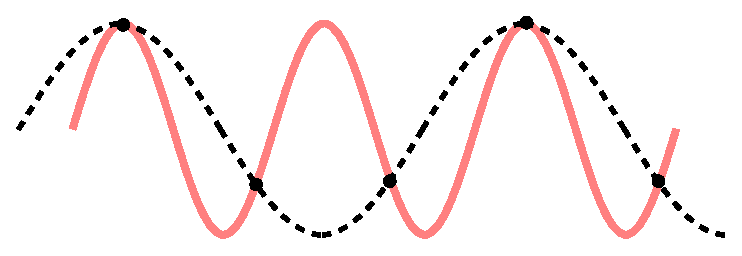
\includegraphics[width = 0.5\textwidth]{figs/alias}
\end{figure}

\section{The Heisenberg uncertainty principle}
[From \S5.4 of \cite{SteinShakarchi_03}] Suppose $\psi$ is a Schwartz function which satisfies the normalizing condition
\begin{align}
    \int_\infty^\infty |\psi(x)|^2 \;\de x = 1.\label{eq:normaliz}
\end{align}

\subsection{}
Show that
\begin{align}
    \left( \int_\infty^\infty x^2|\psi(x)|^2 \;\de x \right)\left( \int_\infty^\infty \xi^2|\hat\psi(\xi)|^2 \;\de \xi \right) \geq \frac{1}{16\pi^2}.
\end{align}
In fact, we have
\begin{align}
    \left( \int_\infty^\infty (x-x_0)^2|\psi(x)|^2 \;\de x \right)\left( \int_\infty^\infty (\xi-\xi_0)^2|\hat\psi(\xi)|^2 \;\de \xi \right) \geq \frac{1}{16\pi^2}.
\end{align}

Hint: start from \eqref{eq:normaliz}, integrate by parts. Remember to use the Cauchy-Schwarz inequality and the Plancherel formula (Parseval identity). 

Remark: You might recognize $|\psi(x)|^2$ as a probability distribution and we have the variance of $|\psi(x)|^2$ and $|\hat\psi(\xi)|^2$. The interpretation of this result in quantum mechanics is:
\begin{align}
    \text{(uncertainty of position)}\times\text{(uncertainty of momentum)} \geq \frac{\hbar}{16\pi^2}
\end{align}
where $\hbar$ is the Planck's constant. If you know a bit of quantum mechanics or is interested, I encourage you to work through Problem 5.23 of \cite{SteinShakarchi_03}. 

\subsection{}
[From Problem 5.21 of \cite{SteinShakarchi_03}] Another statement of the uncertainty principle is: suppose that $f$ is continuous on $\mathbb{R}$. Show that $f$ and $\hat f$ cannot both be compactly supported unless $f = 0$. 

Hint: Assume $f$ is supported in $[0, 1/2]$. Expand $f$ in a Fourier series in the
interval $[0, 1]$, and note that as a result, $f$ is a trigonometric polynomial.



\vfill
\printbibliography


\end{document}